\subsubsection{Running time and speed-up.}

Table~\ref{tbl:parallelTimes} shows the wall clock times achieved by
{\tt psta}, {\tt libcds}, and {\tt sdsl} on different inputs.
Each time is the minimum achieved over three non-consecutive runs, reflecting
our assumption that slightly increased running times are the result of
``noise'' from external processes such as operating system and networking tasks.
Figure~\ref{fig:speedup} shows the speed-up for the {\tt ctree} and {\tt osm}
inputs compared to the running times of {\tt psta} on a single core and
of {\tt sdsl}.

The {\tt psta} algorithm on a single core and {\tt sdsl} outperformed
{\tt libcds} by an order of magnitude.  One of the reasons for this is
that {\tt libcds} implements a different version of {\tt RMMT}
including {\em rank} and {\em select} structures, while {\tt psta} and
{\tt sdsl} do not.  Constructing these structures is costly.  On a
single core, {\tt sdsl} was about 1.5 times faster than {\tt psta},
but neither {\tt sdsl} nor {\tt libcds} were able to take advantage of
multiple cores, so {\tt psta} outperformed both of them starting at
$p = 2$.  The advantage of {\tt sdsl} over {\tt psta} on a single
core, in spite of implementing essentially the same algorithm, can be
attributed to (1) lack of tuning of {\tt psta} and (2) some overhead
with running parallel code on a single core.

\begin{figure}[t]
  \begin{minipage}[b]{0.47\textwidth}
    \setlength{\tabcolsep}{0pt}
    \begin{tabular}{c@{\hspace{1em}}r@{ }r@{ }r@{ }r@{ }r}
      \toprule
      $p$ & {\tt wiki} & {\tt prot} & {\tt dna} & {\tt ctree} & {\tt osm}\\
      \midrule
      {\tt libcds} & 33.16 & 44.24 & 75.87 & 140.41 & 339.21 \\
      {\tt sdsl} & 1.93 & 2.66 & 4.57 & 8.35 & 18.10 \\
      \midrule
      1 & 2.89 & 4.22 & 7.21 & 12.16 & 30.60 \\
      2 & 1.44 & 2.13 & 3.64 & 6.15 & 15.43 \\
      4 &  .73 & 1.10 & 1.87 & 3.18 & 7.98 \\
      8 &  .37 &  .57 &  .98 & 1.59 & 4.14 \\
      16 &  .25 &  .35 &  .58 &  .86 & 2.21 \\
      32 &  .18 &  .25 &  .39 &  .63 & 1.33 \\
      64 &  .27 &  .29 &  .39 &  .48 & 1.01 \\
      \bottomrule
    \end{tabular}
  \end{minipage}%
  \hspace{\stretch{1}}%
  \begin{minipage}[c]{0.5\textwidth}
    \leavevmode\rlap{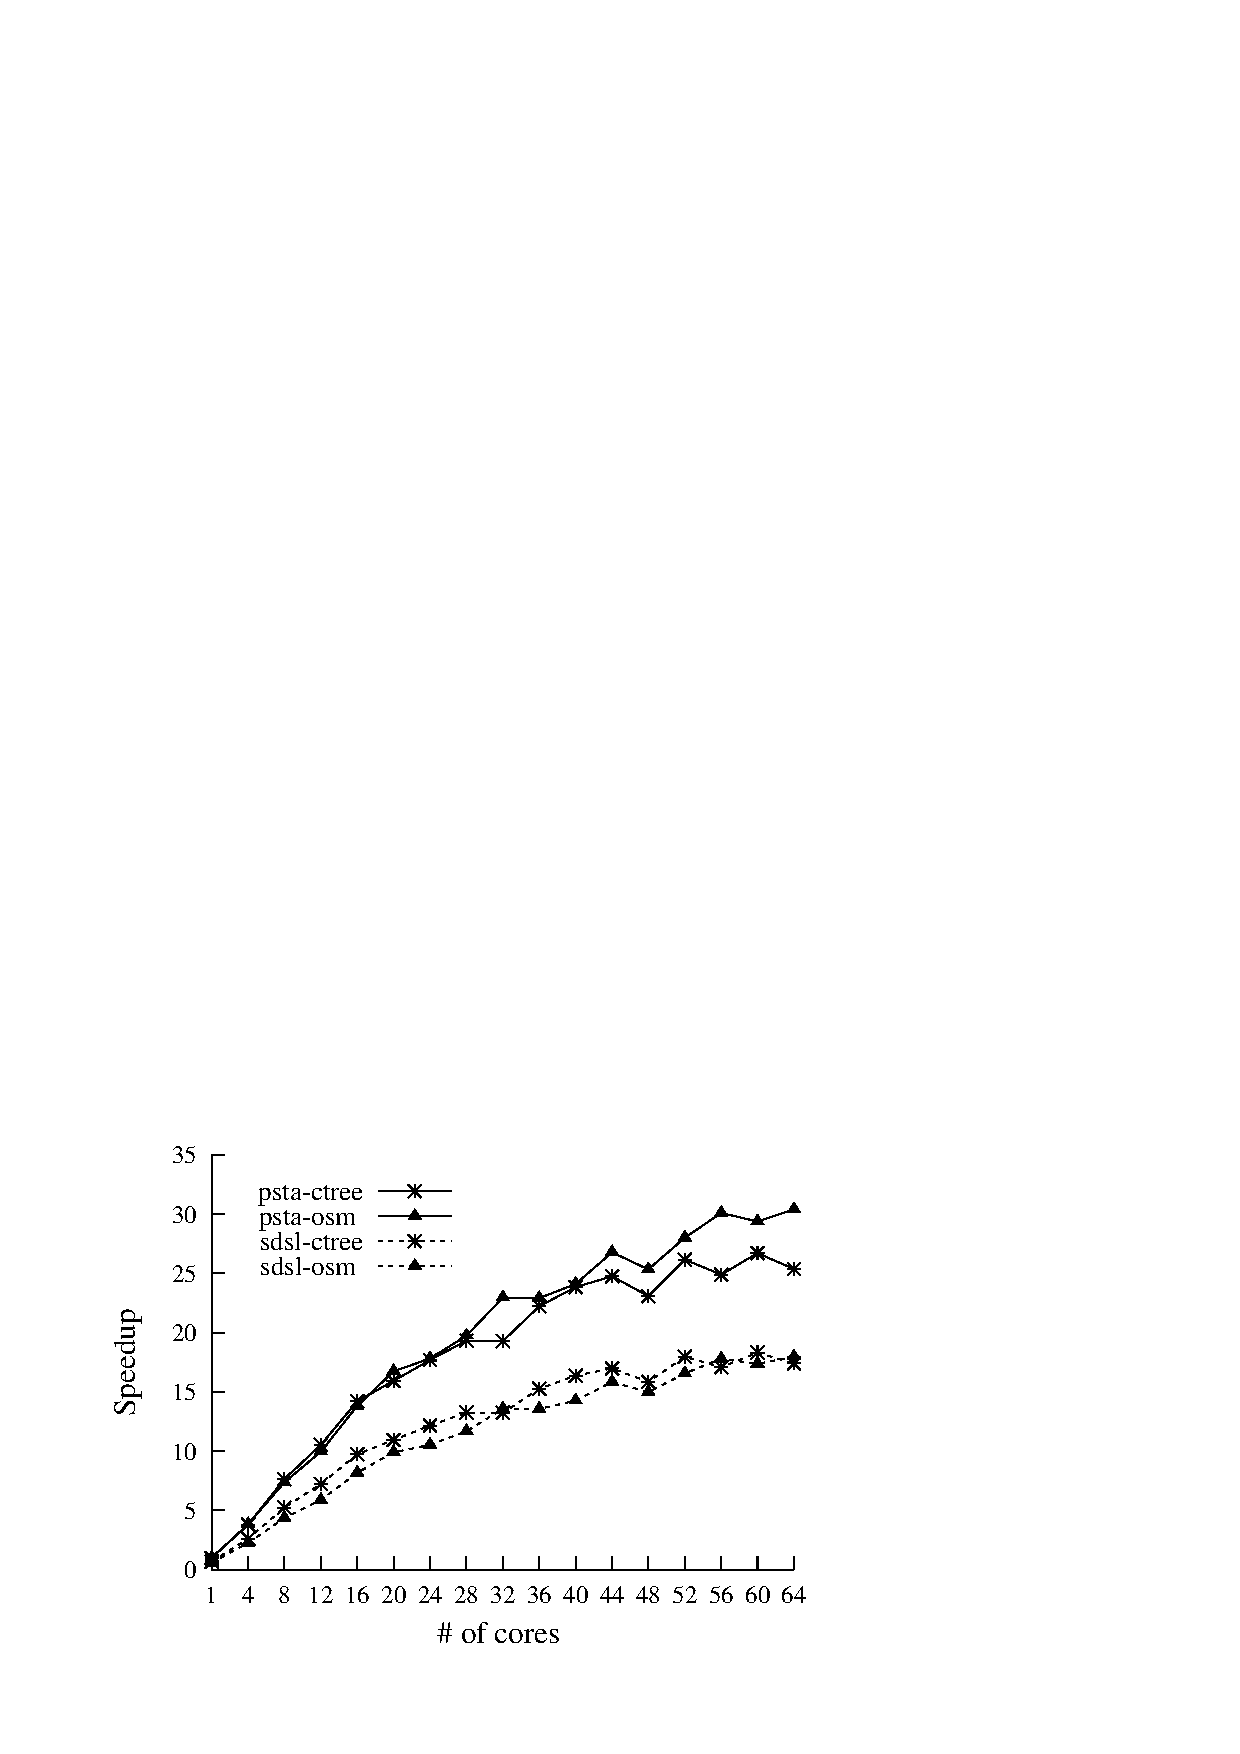
\includegraphics[width=1.04\textwidth]{./images/speedup}}
  \end{minipage}\\[1ex]
  \leavevmode\begin{minipage}[t]{0.47\textwidth}
    \captionof{table}{Running times of {\tt PSTA}, {\tt libcds}, and {\tt sdsl}
      in seconds.\label{tbl:parallelTimes}}
  \end{minipage}%
  \hspace{\stretch{1}}%
  \begin{minipage}[t]{0.5\textwidth}
    \captionof{figure}{Speed-up on {\tt ctree} and {\tt osm}
      data sets.\label{fig:speedup}}
  \end{minipage}
\end{figure}

Up to 16 cores, the speed-up of {\tt psta} is almost linear whenever $p$ is a
power of $2$ and the efficiency (speed-up/$p$) is 70\% or higher, except for
{\tt ctree} on 32 cores.
This is very good for a multicore architecture.
When $p$ is not a power of~$2$, speed-up is slightly worse.
The reason is that, when $p$ is a power of $2$, {\tt psta} can assign exactly
one subtree to each thread (see Algorithm \ref{algo:PSTA2}), distributing the
work homogeneously across cores without any work stealing.
When the number of threads is not a power of two, some threads have to process
more than one subtree and other threads process only one, which degrades
performance due to the overhead of work stealing.

There were three other factors that limited the performance of {\tt psta} in
our experiments: network topology, input size, and resource contention with
the OS.

\textit{Topology.}
The four processors on our machine were connected in a grid
topology~\cite{Drepper2007}.
Up to 32 threads, all threads can be run on a single processor or on two
adjacent processors in the grid, which keeps the cost of communication between
threads low.
Beyond 32 threads, at least three processor are needed and
at least two of them are not adjacent in the grid.
This increases the cost of communication between threads on these processors
noticeably.

\textit{Input size.}
For the two largest inputs we tested, {\tt osm} and {\tt ctree}, speed-up
kept increasing as we added more cores.
For {\tt wiki}, however, the best speed-up was achieved with 36 cores.
Beyond this, the amount of work to be done per thread was small enough that
the scheduling overhead caused by additional threads started to outweigh the
benefit of reducing the processing time per thread further.

\textit{Resource contention.}
For $p < 64$, at least one core on our machine was available to OS processes,
which allowed the remaining cores to be used exclusively by {\tt psta}.
For $p = 64$, {\tt psta} competed with the OS for available cores.
This had a detrimental effect on the efficiency of {\tt psta} for $p = 64$.

\subsubsection{Memory usage.}
We measured the amount of working memory (i.e., memory not occupied by the raw
parenthesis sequence) used by {\tt psta}, {\tt libcds}, and {\tt sdsl}.
We did this by monitoring how much memory was allocated/released with
\texttt{malloc}/\texttt{free} and recording the peak usage.
For {\tt psta}, we only measured the memory usage for $p = 1$.
The extra memory needed for thread scheduling when $p > 1$ was negligible.
Due to lack of space, we report the results only for the two largest inputs,
{\tt ctree} and {\tt osm}.
For the {\tt ctree} input, {\tt psta}, {\tt libcds}, and {\tt sdsl} used 112MB,
38MB, and 76MB of memory, respectively.
For {\tt osm}, they used 331MB, 85MB, and 194MB, respectively.
Even though {\tt psta} uses more memory than both {\tt libcds} and {\tt sdsl},
the difference between {\tt psta} and {\tt sdsl} is a factor of less than two.
The difference between {\tt psta} and {\tt libcds} is no more than a factor of
four and is outweighed by the substantially worse performance of {\tt libcds}.

Part of the higher memory usage of {\tt psta} stems from the allocation of
$e^{\prime}$, $m^{\prime}$, $M^{\prime}$ and $n^{\prime}$ arrays to store the
partial excess values in the algorithm.
Storing these values, however, is a key factor that helps {\tt psta} to achieve
very good performance.
